\documentclass[12pt,a4paper]{article}
\usepackage{amsmath}
\usepackage{algorithm}
\usepackage{algpseudocode}
\usepackage{graphics}
\usepackage{graphicx}
\usepackage[normalem]{ulem}
\usepackage[table,xcdraw]{xcolor}
\usepackage{grffile,graphicx,hyperref,graphbox}
\usepackage{fancyhdr}
\usepackage{listings}
\usepackage{array}
\usepackage[top=1in,headsep=4pt,headheight=26pt,bottom=1.in,left=1in,right=1in]{geometry}
\usepackage{lipsum}
\usepackage{sectsty}
\usepackage{subcaption}
\usepackage{times}
\sectionfont{\large \color[HTML]{cc3333}}
\usepackage{multirow}
\usepackage{tabularx}
\usepackage{geometry}
\usepackage{longtable}
\usepackage{makecell}
\usepackage{ltablex}
\usepackage[font=footnotesize]{caption}
\usepackage{tikz}
\usetikzlibrary{arrows.meta}
\keepXColumns
\usepackage{amsmath}
\usepackage{amssymb}

\usepackage[
backend=biber,
style=numeric,
]{biblatex}
\addbibresource{example_paper.bib}

\usepackage{algpseudocode}
\algtext*{EndIf}
\algtext*{EndFor}

\usepackage[linewidth=1pt]{mdframed}
\setlength\parindent{0pt}

\fancypagestyle{firststyle}
{
   \fancyhf{}
   \lhead{
\includegraphics[width=5cm]{image4.png}}
}

\title{\large{Algorithms and Analysis Report}
\\
COSC2123/3119
\\
Graph Algorithms in Action: Modelling a Disease Outbreak
} \vspace{-0.2cm}
\author{Your Name and Student Number Here}
\date{}

\begin{document}
\maketitle
\thispagestyle{firststyle}
\vspace{-1cm}

\begin{table}[h]
\begin{tabular}{|l|p{11cm}|}
\hline
{\color[HTML]{cc3333} Assessment Type} & Individual assignment. Submit online via GitHub. \\ \hline
{\color[HTML]{cc3333} Due Date}        & Week 11, Thursday May 21, 13:00 (1pm). A late penalty will apply to assessments submitted after 13:00. \\ \hline
{\color[HTML]{cc3333} Marks}           & 30 \\ \hline
\end{tabular}
\end{table}

\vspace{-0.7cm}
\section{Learning Outcomes}

This assessment relates to four learning outcomes of the course which are:
\begin{itemize}
    \item CLO 1: Compare, contrast, and apply the key algorithmic design paradigms: brute force, divide and conquer, decrease and conquer, transform and conquer, greedy, dynamic programming and iterative improvement;
    \item CLO 2: Compare, contrast, and apply key data structures: trees, lists, stacks, queues, hash tables and graph representations;
    \item CLO 3: Define, compare, analyse, and solve general algorithmic problem types: sorting, searching, graphs and geometric;
    \item CLO 4: Theoretically compare and analyse the time complexities of algorithms and data structures; and
    \item CLO 5: Implement, empirically compare, and apply fundamental algorithms and data structures to real-world problems.
\end{itemize}

\vspace{-0.4cm}
\section{Overview}

Across multiple tasks in this assignment, you will model a disease outbreak in the city of
Metropolis as a weighted graph to capture residents' contacts, implement and compare algorithms
for estimating infection risk through the population, and design a dynamic programming strategy
to allocate scarce antiviral treatment as effectively as possible. Some components ask you to
critically assess your solutions through both theoretical analysis and controlled empirical
experiments, encouraging reflection on the relationship between algorithm design and real-world
performance.

\begin{quote}
\begin{mdframed}
\emph{I certify that this is all my own original work. If I took any parts from elsewhere,
then they were non-essential parts of the assignment, and they are clearly attributed in my
submission. I will show I agree to this honor code by typing ``Yes'': YOUR ANSWER HERE}
\end{mdframed}
\end{quote}

\newpage

\section{Motivation}

The T-Virus has broken out in the city of Metropolis. As the newly 
appointed Regional Health Director, you have been handed a dossier 
containing everything the epidemiologists know: a map of every known 
contact between residents, the probability that each contact transmits 
the virus in a single day, and the vulnerability of each resident. 
The clock is ticking --- every day the virus spreads further, and your 
antiviral stockpile is limited. \\

Your job has four parts:
\begin{enumerate}
    \item \textbf{Build the contact network} (Task A) --- represent 
          the city's contact relationships as a graph, efficiently 
          enough to run algorithms on in real time (implement \\ \texttt{graph/adjacency\_matrix.py}).
    \item \textbf{Estimate infection risk} (Task B) --- compute the 
          probability that each resident becomes infected over the 
          coming $T$ days, identifying the most at-risk residents 
          before the outbreak grows (implement \texttt{transmission/task\_b.py} and write report).
    \item \textbf{Analyse your solution} (Task C) --- theoretically 
          and empirically compare your algorithm against the provided 
          baseline across different network structures (write report on analysis of task A and B).
    \item \textbf{Allocate antiviral treatment} (Task D) --- decide 
          who receives the scarce supply of doses, maximising 
          the benefit to the population within the limits of your 
          stockpile (implement \texttt{treatment/task\_b.py} and write report).
\end{enumerate}

Figure~\ref{fig:village} shows the contact network for sub-population in Metropolis. 
Each resident is a node, and each contact relationship is an edge 
labelled with the daily probability of transmission. Patient zero 
$V_0$ is already infected --- the question is how far the virus will 
spread, and who we should protect first.

\begin{figure}[H]
\centering
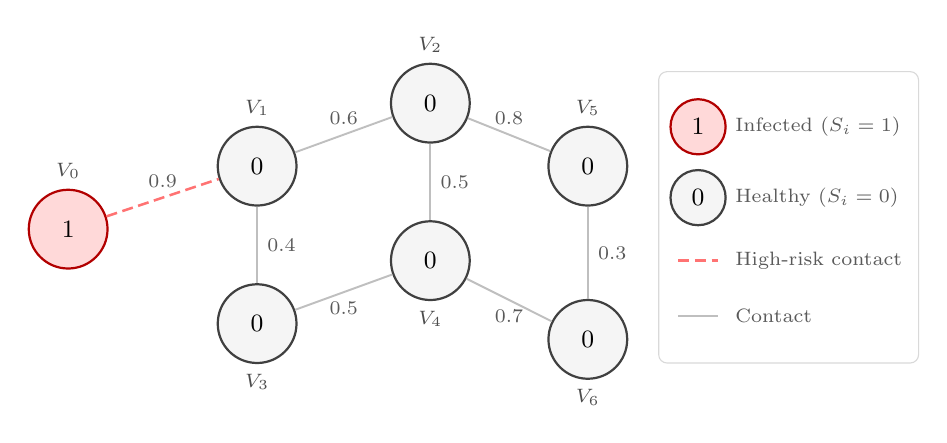
\begin{tikzpicture}[
    every node/.style={font=\small},
    infected/.style={circle, draw=red!70!black, fill=red!15,
        line width=0.8pt, minimum size=10mm, inner sep=0pt},
    healthy/.style={circle, draw=gray!50!black, fill=gray!8,
        line width=0.8pt, minimum size=10mm, inner sep=0pt},
    contact/.style={draw=gray!50, line width=0.7pt},
    highrisk/.style={draw=red!55, line width=0.9pt, dashed,
        dash pattern=on 4pt off 2pt},
    lbl/.style={font=\scriptsize\color{gray!70!black}}
]
\node[infected, label={[font=\scriptsize,gray!60!black]above:$V_0$}]
    (v0) at (0.0,  0.0) {1};
\node[healthy, label={[font=\scriptsize,gray!60!black]above:$V_1$}]
    (v1) at (2.4,  0.8) {0};
\node[healthy, label={[font=\scriptsize,gray!60!black]above:$V_2$}]
    (v2) at (4.6,  1.6) {0};
\node[healthy, label={[font=\scriptsize,gray!60!black]below:$V_3$}]
    (v3) at (2.4, -1.2) {0};
\node[healthy, label={[font=\scriptsize,gray!60!black]below:$V_4$}]
    (v4) at (4.6, -0.4) {0};
\node[healthy, label={[font=\scriptsize,gray!60!black]above:$V_5$}]
    (v5) at (6.6,  0.8) {0};
\node[healthy, label={[font=\scriptsize,gray!60!black]below:$V_6$}]
    (v6) at (6.6, -1.4) {0};
\draw[highrisk] (v0) -- node[above, lbl]{0.9} (v1);
\draw[contact]  (v1) -- node[above, lbl]{0.6} (v2);
\draw[contact]  (v1) -- node[right, lbl]{0.4} (v3);
\draw[contact]  (v2) -- node[above, lbl]{0.8} (v5);
\draw[contact]  (v3) -- node[below, lbl]{0.5} (v4);
\draw[contact]  (v4) -- node[below, lbl]{0.7} (v6);
\draw[contact]  (v5) -- node[right, lbl]{0.3} (v6);
\draw[contact]  (v2) -- node[right, lbl]{0.5} (v4);
\draw[draw=gray!30, fill=white, rounded corners=3pt]
    (7.5, -1.7) rectangle (10.8, 2.0);
\node[infected, minimum size=7mm] at (8.0,  1.3) {1};
\node[anchor=west, font=\scriptsize, gray!70!black]
    at (8.35, 1.3) {Infected ($S_i=1$)};
\node[healthy, minimum size=7mm] at (8.0,  0.4) {0};
\node[anchor=west, font=\scriptsize, gray!70!black]
    at (8.35, 0.4) {Healthy ($S_i=0$)};
\draw[highrisk] (7.75,-0.4) -- (8.25,-0.4);
\node[anchor=west, font=\scriptsize, gray!70!black]
    at (8.35,-0.4) {High-risk contact};
\draw[contact]  (7.75,-1.1) -- (8.25,-1.1);
\node[anchor=west, font=\scriptsize, gray!70!black]
    at (8.35,-1.1) {Contact};
\end{tikzpicture}
\caption{The contact network $G = (V, E)$ for Metropolis. $V_0$ 
is patient zero. Edge labels give the daily transmission 
probability $w_{ij} \in (0,1]$. Dashed red edges originate from 
an infected resident.}
\label{fig:village}
\end{figure}

By vaccinating even a small number of strategically chosen 
residents, we can sever the most dangerous transmission pathways 
through the network. Figure~\ref{fig:vaccination} shows an 
example: vaccinating $V_1$ --- the single resident through whom 
all transmission from $V_0$ must pass --- protects every 
downstream resident at once.

\begin{figure}[H]
\centering
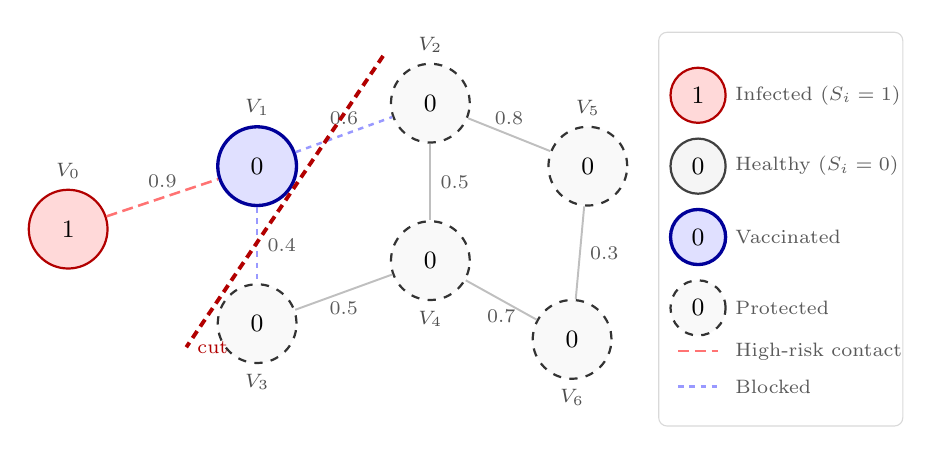
\begin{tikzpicture}[
    every node/.style={font=\small},
    infected/.style={circle, draw=red!70!black, fill=red!15,
        line width=0.8pt, minimum size=10mm, inner sep=0pt},
    healthy/.style={circle, draw=gray!50!black, fill=gray!8,
        line width=0.8pt, minimum size=10mm, inner sep=0pt},
    vaccinated/.style={circle, draw=blue!60!black, fill=blue!12,
        line width=1.2pt, minimum size=10mm, inner sep=0pt},
    protected/.style={circle, draw=gray!40!black, fill=gray!5,
        line width=0.8pt, minimum size=10mm, inner sep=0pt, dashed},
    contact/.style={draw=gray!50, line width=0.7pt},
    highrisk/.style={draw=red!55, line width=0.9pt, dashed,
        dash pattern=on 4pt off 2pt},
    blocked/.style={draw=blue!40, line width=0.9pt, dashed,
        dash pattern=on 2pt off 2pt},
    lbl/.style={font=\scriptsize\color{gray!70!black}}
]
\node[infected, label={[font=\scriptsize,gray!60!black]above:$V_0$}]
    (v0) at (0.0,  0.0) {1};
\node[vaccinated, label={[font=\scriptsize,gray!60!black]above:$V_1$}]
    (v1) at (2.4,  0.8) {0};
\node[protected, label={[font=\scriptsize,gray!60!black]above:$V_2$}]
    (v2) at (4.6,  1.6) {0};
\node[protected, label={[font=\scriptsize,gray!60!black]below:$V_3$}]
    (v3) at (2.4, -1.2) {0};
\node[protected, label={[font=\scriptsize,gray!60!black]below:$V_4$}]
    (v4) at (4.6, -0.4) {0};
\node[protected, label={[font=\scriptsize,gray!60!black]above:$V_5$}]
    (v5) at (6.6,  0.8) {0};
\node[protected, label={[font=\scriptsize,gray!60!black]below:$V_6$}]
    (v6) at (6.4, -1.4) {0};
\draw[highrisk] (v0) -- node[above, lbl]{0.9} (v1);
\draw[blocked]  (v1) -- node[above, lbl]{0.6} (v2);
\draw[blocked]  (v1) -- node[right, lbl]{0.4} (v3);
\draw[contact]  (v2) -- node[above, lbl]{0.8} (v5);
\draw[contact]  (v3) -- node[below, lbl]{0.5} (v4);
\draw[contact]  (v4) -- node[below, lbl]{0.7} (v6);
\draw[contact]  (v5) -- node[right, lbl]{0.3} (v6);
\draw[contact]  (v2) -- node[right, lbl]{0.5} (v4);
\draw[line width=1.4pt, red!70!black, dash pattern=on 3pt off 2pt]
    (4, 2.2) -- (1.5, -1.5)
    node[right, font=\scriptsize, red!70!black] {cut};
\draw[draw=gray!30, fill=white, rounded corners=3pt]
    (7.5, -2.5) rectangle (10.6, 2.5);
\node[infected,   minimum size=7mm] at (8.0,  1.7) {1};
\node[anchor=west, font=\scriptsize, gray!70!black]
    at (8.35, 1.7) {Infected ($S_i=1$)};
\node[healthy,    minimum size=7mm] at (8.0,  0.8) {0};
\node[anchor=west, font=\scriptsize, gray!70!black]
    at (8.35, 0.8) {Healthy ($S_i=0$)};
\node[vaccinated, minimum size=7mm] at (8.0, -0.1) {0};
\node[anchor=west, font=\scriptsize, gray!70!black]
    at (8.35,-0.1) {Vaccinated};
\node[protected,  minimum size=7mm] at (8.0, -1.0) {0};
\node[anchor=west, font=\scriptsize, gray!70!black]
    at (8.35,-1.0) {Protected};
\draw[highrisk] (7.75,-1.55) -- (8.25,-1.55);
\node[anchor=west, font=\scriptsize, gray!70!black]
    at (8.35,-1.55) {High-risk contact};
\draw[blocked]  (7.75,-2.0) -- (8.25,-2.0);
\node[anchor=west, font=\scriptsize, gray!70!black]
    at (8.35,-2.0) {Blocked};
\end{tikzpicture}
\caption{Vaccinating $V_1$ --- the single bottleneck through 
whom all transmission from $V_0$ must pass --- severs every 
onward pathway at once, protecting $V_2$ through $V_6$ entirely. 
This illustrates the core challenge of Task~D: identifying which 
residents to vaccinate in order to maximise protection across 
the network given a limited supply of doses.}
\label{fig:vaccination}
\end{figure}

\subsection{Mathematical Background}

We model the city of Metropolis as a weighted undirected graph 
$G = (V, E)$, where:
\begin{itemize}
    \item each vertex $V_i \in V$ represents a resident, with 
          infection state $S_i \in \{0, 1\}$ where $S_i = 0$ 
          is healthy and $S_i = 1$ is infected;
    \item each edge $(V_i, V_j) \in E$ represents a contact 
          relationship between two residents; and
    \item each edge carries a weight $w_{ij} \in (0, 1]$, 
          the probability that an infected resident $V_i$ 
          transmits the virus to a healthy neighbour $V_j$ 
          in a single day.
\end{itemize}

Each resident $V_i$ also has two personal attributes relevant 
to the vaccine allocation in Task~D:
\begin{itemize}
    \item a \textbf{dosage requirement} $c_i \in \mathbb{Z}^+$, 
          the number of antiviral doses required to vaccinate 
          resident $V_i$; and
    \item a \textbf{vulnerability score} $\phi_i \in (0, 1]$, 
          reflecting how severely resident $V_i$ would be 
          harmed if infected.
\end{itemize}

Once infected, a resident remains infectious forever. Over a 
planning horizon of $T$ days, the probability that an infected 
resident $V_i$ infects neighbour $V_j$ at least once is:
\[
    p_{ij} = 1 - (1 - w_{ij})^{\,T}
\]
As $T \to \infty$, $p_{ij} \to 1$ for any $w_{ij} > 0$ --- 
given enough time, every resident reachable from patient zero 
will eventually be infected. This makes early intervention 
critical. The benefit of vaccinating resident $V_i$ is therefore 
a function of how likely they are to be infected, how severely 
they would be harmed, and how much onward transmission they 
would cause --- all of which are computed from $G$, $r_{i,T}$, 
and $\phi_i$ in Tasks B and D.

\newpage

%%=============================================================
\section*{Task B: Estimating Infection Risk Over Time (7 marks, 1 page)}
%%=============================================================

\subsection*{Pseudo-code}

%%% Replace this example with your own pseudo-code for the DP solution.
%%% Use Algorithm 1 (MonteCarlo) from the assignment spec as a style guide.

The Monte Carlo baseline (Algorithm 1) is provided as a style guide. Write your pseudo-code for the dynamic programming solution below in the same style.

\begin{algorithm}
\caption{MonteCarlo$(G,\ s,\ T,\ X)$}
\label{alg:mc}
\begin{algorithmic}[1]
\Require Graph $G = (V, E)$; source $s$; horizon $T$; simulations $X$
\Ensure Estimated risk table where $\text{table}[t][i] \approx r_{i,t}$
\For{each day $t = 1$ to $T$}
    \For{each simulation $x = 1$ to $X$}
        \State Restart from scratch --- only $s$ is infected
        \For{each day $d = 1$ to $t$}
            \For{each uninfected resident $V_i$}
                \For{each infected neighbour $V_j$ of $V_i$}
                    \State Infect $V_i$ with probability $w_{ij}$
                \EndFor
            \EndFor
        \EndFor
    \EndFor
    \State $\text{table}[t][i] \gets$ fraction of simulations where $V_i$ infected
\EndFor
\State \Return table
\end{algorithmic}
\end{algorithm}

\subsection*{Limitations of the Recurrence}

%%% Answer parts (a), (b), and (c) here.
%%% Reference Figure 5 from the assignment spec in part (b).
%%% Maximum 1 page for the full Task B report.

\begin{enumerate}
    \item[(a)] \textit{Your answer to part (a) here.}
    \item[(b)] \textit{Your answer to part (b) here, with reference to Figure 5.}
    \begin{figure}[h!]
\centering
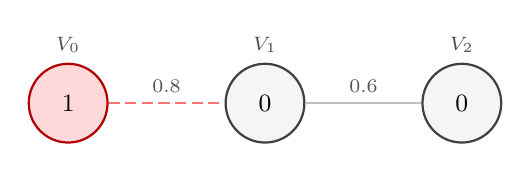
\begin{tikzpicture}[
    every node/.style={font=\small},
    infected/.style={circle, draw=red!70!black, fill=red!15, 
                     line width=0.8pt, minimum size=10mm, inner sep=0pt},
    healthy/.style={circle, draw=gray!50!black, fill=gray!8, 
                    line width=0.8pt, minimum size=10mm, inner sep=0pt},
    highrisk/.style={draw=red!55, line width=0.9pt, dashed, 
                     dash pattern=on 4pt off 2pt},
    contact/.style={draw=gray!50, line width=0.7pt},
    lbl/.style={font=\scriptsize, gray!65!black}
]
\node[infected, label={[font=\scriptsize, gray!60!black]above:$V_0$}] 
    (v0) at (0.0, 0) {1};
\node[healthy,  label={[font=\scriptsize, gray!60!black]above:$V_1$}] 
    (v1) at (2.5, 0) {0};
\node[healthy,  label={[font=\scriptsize, gray!60!black]above:$V_2$}] 
    (v2) at (5.0, 0) {0};
\draw[highrisk] (v0) -- node[above, lbl]{0.8} (v1);
\draw[contact]  (v1) -- node[above, lbl]{0.6} (v2);
\end{tikzpicture}
\caption{This is figure 5.}
\label{fig:simple}
\end{figure}
    \item[(c)] \textit{Your answer to part (c) here.}
\end{enumerate}

\newpage

%%=============================================================
\section*{Task C: Analysis of Infection Risk Algorithms (8 marks, 2 pages)}
%%=============================================================

%%% Maximum 2 pages for the full Task C report.

\subsection*{Algorithm Complexity Analysis}

\textit{Your complexity analysis of all four combinations here.}

\subsection*{Empirical Design}

\textit{Describe which variables you vary, which you fix, and why.}

\subsection*{Empirical Analysis}

%%% Include clearly labelled plots comparing all four combinations.
%%% Plots should be generated in Python using matplotlib.

\begin{figure}[H]
    \centering
    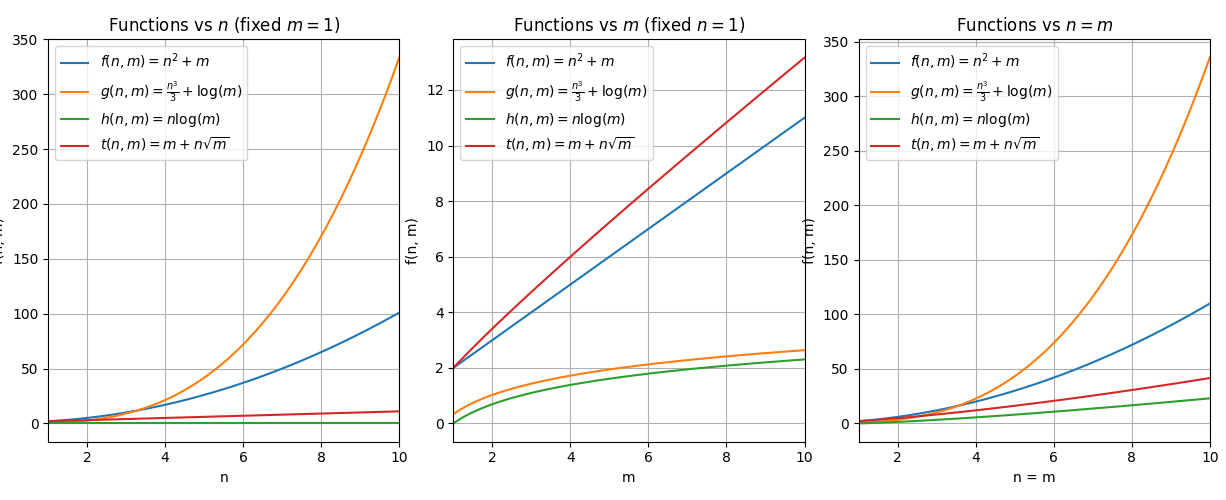
\includegraphics[width=1\linewidth]{img/plot_example.png}
    \caption{Runtime comparison of the four algorithm and representation
    combinations. \textit{Replace this with your own plot and caption.}}
    \label{fig:task_c_plot}
\end{figure}

\subsection*{Reflection}

\textit{Your reflection here, including a recommendation for Metropolis
and a discussion of how your answer would change if transmission rates
and connections updated daily.}

\newpage

%%=============================================================
\section*{Task D: Antiviral Allocation (10 marks, 2 pages)}
%%=============================================================

%%% Maximum 2 pages for the full Task D report.

\subsection*{Algorithm Design}

\textit{Describe the algorithm you designed.}

\subsection*{Complexity Analysis}

\textit{Justify the time complexity of your solution. Explain where each
factor comes from.}

\subsection*{Extension 1: Triage}

\textit{Describe how you would modify your solution to handle $K$
vulnerability tiers. State the complexity of your modified solution.
Include a small numerical counterexample showing that ignoring
vulnerability can lead to a highly vulnerable resident being passed
over.}

\subsection*{Extension 2: Interdependent Vaccinations}

\textit{Explain why the independence assumption $b_i = r_{i,T}$ is
necessary for your solution to be valid. Construct a small example showing
that ignoring interdependence leads to a sub-optimal outcome. Explain
why the true optimal problem under interdependence is significantly
harder to solve.}

%%% If you make any claims based on external sources, cite them.
\printbibliography

\end{document}